\chapter{Metodologia}
\section{Sistemas simulados}\label{SistemasSimulados}

Simulações de dinâmica molecular foram efetuadas utilizando os dendrímeros Poli(amido amina) (PAMAM) com núcleo de etileno diamina (EDA) e Poli(propileno imina) (PPI) com núcleo de 1,4-diamino butano (DAB) de gerações 0 até 5 e 1 à 6, respectivamente, considerando condições de pH alto($pH > 10.0$), neutro($pH \sim 7.1$) e baixo($pH < 4.0$).
A tabela \ref{tab:sistemas} reporta os 36 sistemas simulados explicitando o número de átomos no dendrímero, de contra-íons e de moléculas de solvente.

A escolha de uma faixa diferente de gerações para o PAMAM e o PPI (também conhecido como Astramol\cite{Kabanov1999}) é devido à nomenclatura utilizada pela literatura para cada um dos dendrímeros ser distinta.
As gerações foram escolhidas de forma que houvessem o mesmo número de grupos terminais para ambas as estruturas.

\begin{table}[ht]
\centering
    \begin{tabular}{ccccc|ccccc}
    \hline
    \multicolumn{5}{c|}{PAMAM} & \multicolumn{5}{c}{PPI} \\
    \hline
    Gen.    &  pH  &    \#Atoms    &    \#Cl$^{-}$ &    \#Water & Gen.      &  pH  &    \#Atoms    &    \#Cl$^{-}$ &    \#Water    \\
    \hline
    G0  &  \multirow{6}{*}{Low}  &   54      &   6   &   1674    & G1     &  \multirow{6}{*}{Low}&   36      &   6   &   1348\\
    G1  &    &   142     &   14  &   4292    & G2     &  &   84      &   14  &   2921\\
    G2  &    &   348     &   30  &   11803   & G3     &  &   180     &   30  &   5257\\
    G3  &    &   670     &   62  &   10394   & G4     &  &   372     &   62  &   8486\\
    G4  &    &   1374    &   126 &   19248   & G5     &  &   756     &   126 &   13075\\
    G5  &    &   2782    &   254 &   36214   & G6     &  &   1524    &   254 &   23546\\
    \hline 
    G0  &  \multirow{6}{*}{Neutral} &    52      &   4   &   1666    & G1     &  \multirow{6}{*}{Neutral}&   34      &   4   &   1140\\
    G1  &  &    136     &   8   &   4033    & G2     &  &    78      &   10  &   2416\\
    G2  &  &    304     &   16  &   8550    & G3     &  &    172     &   22  &   3593\\
    G3  &  &    640     &   32  &   13241   & G4     &  &    356     &   46  &   5014\\
    G4  &  &    1312    &   64  &   17982   & G5     &  &    724     &   94  &   9723\\
    G5  &  &    2656    &   128 &   34096   & G6     &  &    1460    &   190 &   14865\\
    \hline
    G0  &  \multirow{6}{*}{High}&   48      &   0   &   1348    & G1     &  \multirow{6}{*}{High}&    30      &   0   &   1143\\
    G1  &  &   128     &   0   &   3653    & G2     &  &   70      &   0   &   1482\\
    G2  &  &   288     &   0   &   8281    & G3     &  &   150     &   0   &   2258\\
    G3  &  &   608     &   0   &   15943   & G4     &  &   310     &   0   &   3213\\
    G4  &  &   1248    &   0   &   14713   & G5     &  &   630     &   0   &   4136\\
    G5  &  &   2528    &   0   &   23565   & G6     &  &   1270    &   0   &   6351\\
    \hline
    \end{tabular}
    \caption{Dimensões dos sistemas considerados nesse trabalho. O número de íons Cl$~{-}$ reportados para o PPI nessa tabela foram calculados considerando a protonação de acordo com o modelo de Ising\cite{VanDuijvenbode1998, Koper1997}.}
    \label{tab:sistemas}
\end{table} 

As condições de pH foram levadas em conta considerando os estados de protonação propostos por Cakara \textit{et al}\cite{Cakara2003}: Em pH ácido, todas as aminas estão protonadas; em neutro, somente as primárias e em pH baixo nenhuma delas é protonada. 
A Figura \ref{PAMAMProt} ilustra o esquema de protonação utilizado para o PAMAM.
Contudo, ainda não existe um acordo sobre o perfil de protonação do PPI na literatura. 
Por isso, dois estados de protonação diferentes foram considerados para o meio com pH neutro: Um deles supondo uma protonação idêntica à do PAMAM (somente os terminais protonados) e outra considerando que somente a penúltima geração estaria desprotonada, como proposto por trabalhos baseados no modelo de Ising\cite{VanDuijvenbode1998, Koper1997} (Essa ultima será referenciada na Tabela \ref{tab:Rg} como ``NEWPROT'' na Seção \ref{ProtonacaoPPI}).
Resultando em um total de 42 simulações efetuadas.

\begin{figure}[ht]
\centering
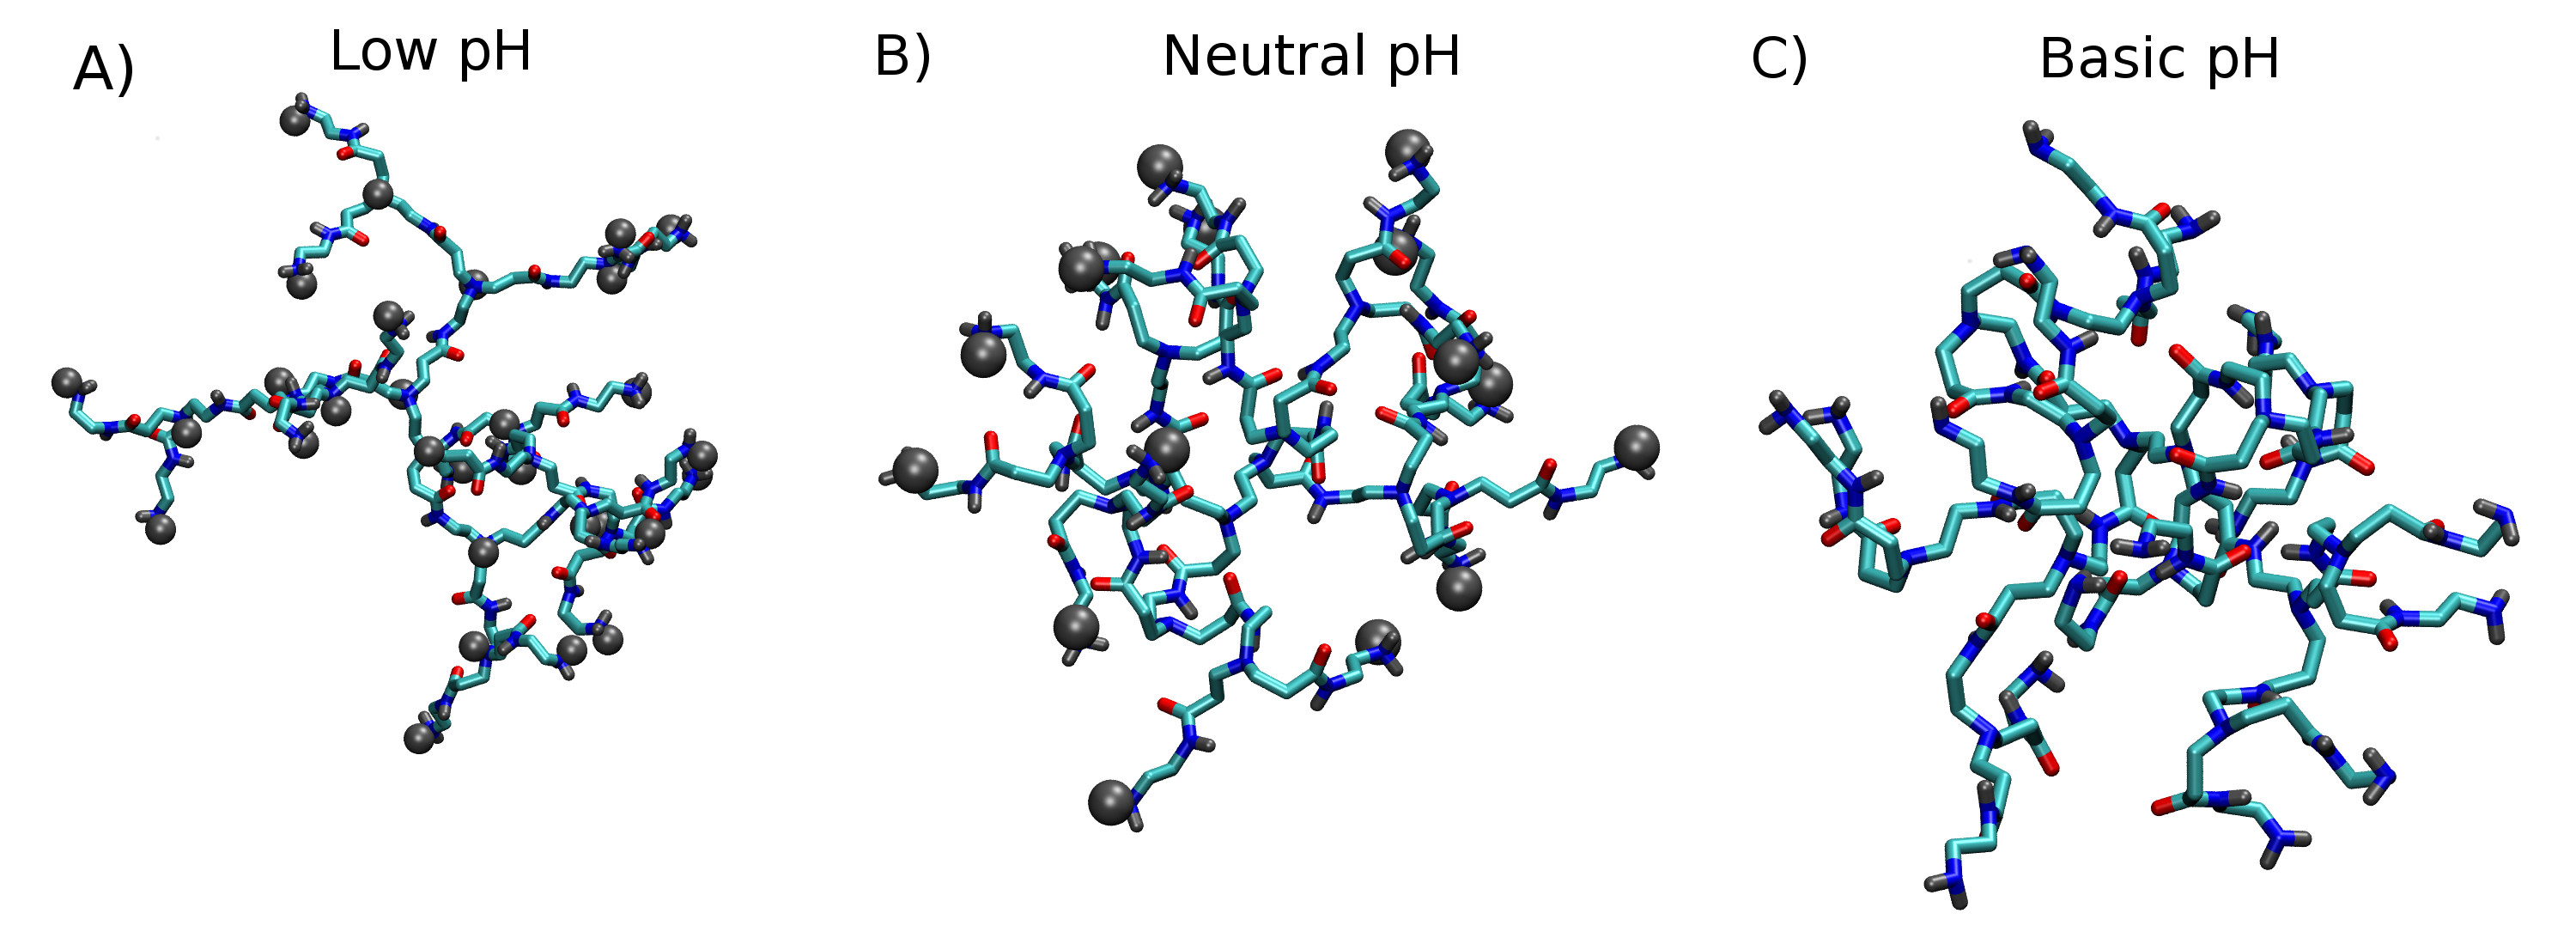
\includegraphics[scale=0.15]{PAMAMProt.png}
\caption{Esquema de protonação do PAMAM de terceira geração. As esferas de van der Waals em cinza representam os hidrogênios inseridos devido ao pH do meio.}
\label{PAMAMProt}
\end{figure}

De fato, o modelo utilizado como base não é determinístico. 
Ele resulta em um grau de protonação dado em percentual do sítio estar protonado ou não.
O estado de protonação sugerido pelos autores\cite{VanDuijvenbode1998, Koper1997} foi um onde cada geração é protonada intercaladamente.
Ou seja, ou todas as gerações pares estarão protonadas ou todas as ímpares.
Isso se deve ao fato de que a protonação de um sítio causa uma repulsão que impede a aproximação de prótons nos sítios de gerações vizinhas.
Mas como o resultado é probabilístico, as curvas de grau de protonação em função do pH estão próximas de 0.5 no estudo reportado\cite{VanDuijvenbode1998, Koper1997}.
Por isso o estado de protonação escolhido foi distinto do proposto no trabalho original aqui citado.
Contudo, veremos à frente que em termos de raio de giro, a diferença não é significativa.

As estruturas iniciais e as topologias foram criadas utilizando o software PyPolyBuilder, criado pelo nosso grupo.
Esse programa se propõe a criar arquivos de estrutura e de topologia para moléculas a partir de blocos de construção menores como foi exposto na Seção \ref{PyPolyBuilder}.


\section{Protocolo de simulação}\label{ProtocoloDeSimulacao}
As simulações de todos os 42 sistemas foram efetuadas utilizando o pacote GROMACS 5.1.4\cite{VanDerSpoel2005} e o campo de força GROMOS-compatible 2016H66\cite{Horta2016}.
As equações de Newton foram integradas usando o algoritmo leap-frog com passo de tempo de 2 fs.
Todas as ligações foram mantidas rígidas segundo o algoritmo LINCS\cite{Hess1997}.
As interações eletrostáticas foram avaliadas com o método PME\cite{Essmann1995} com um raio de corte do espaço real de $1.2$ nm e um espaçamento de malha de $0.12$ nm.

Dois \textit{setups} foram considerados para as interações de Lennard-Jones para avaliar a influência das configurações da simulação utilizando o campo de força 2016H66\cite{Horta2016} no GROMACS, segundo a filosofia do estudo de Gonçalves \textit{et al}\cite{Goncalvez2018}. 
Em uma delas, nomeada de ``CUT'', as interações foram truncadas em $1.2$ nm usando um raio de corte simples, método conhecido como \textit{cut-off}.
Em outra, rotulada como ``PME'', avaliamos as interações segundo o método PME\cite{Essmann1995} com raio de corte do espaço real de $1.2$ nm e espaçamento de malha de $0.12$ nm.
Veremos na Seção \ref{EfeitoDoSetup} que nos sistemas considerados na presente dissertação, a escolha do \textit{setup} não teve grande efeito.
Os resultados são praticamente os mesmos independentemente do método de avaliação das interações de Lennard-Jones.

Vale notar que o protocolo descrito acima não está de acordo com a parametrização do campo de força, mas foi mostrado ser o mais adequado em um estudo sistemático realizado por Gonçalves \textit{et al}\cite{Goncalvez2018}.

Temperatura e pressão foram controladas por acoplamento fraco com um banho externo de calor e de volume segundo o termostato modificado de Berendsen\cite{Berendsen1984, Bussi2007} e o formalismo de Parrinelo-Rahman\cite{Parrinello1981, Andersen1980}, respectivamente.
A constante de tempo do acoplamento térmico foi definida como 0.1 ps e, para o acoplamento de pressão, a constante de tempo e a compressibilidade isotérmica utilizadas foram 2.0 ps e $4.5\times10^{-5}$bar$^{-1}$, respectivamente.

Primeiramente, uma minimização em vácuo foi realizada por 5000 passos e o sistema foi colocado em uma caixa de simulação cúbica de forma que todos os átomos estivessem, no mínimo, a $1$ nm de distância das faces dessa caixa.
O sistema foi então solvatado com uma quantidade suficientemente grande de moléculas de água SPC\cite{Berendsen1981}.
Nos casos onde a carga total do sistema não fosse neutra, o sistema foi neutralizado pela adição de contra-íons Cl$^{-}$ (para mais informações, veja a Tabela \ref{tab:sistemas}).
Após a solvatação, uma nova etapa de minimização de energia foi feita considerando condições de contorno periódicas.

\begin{figure}[ht]
\centering
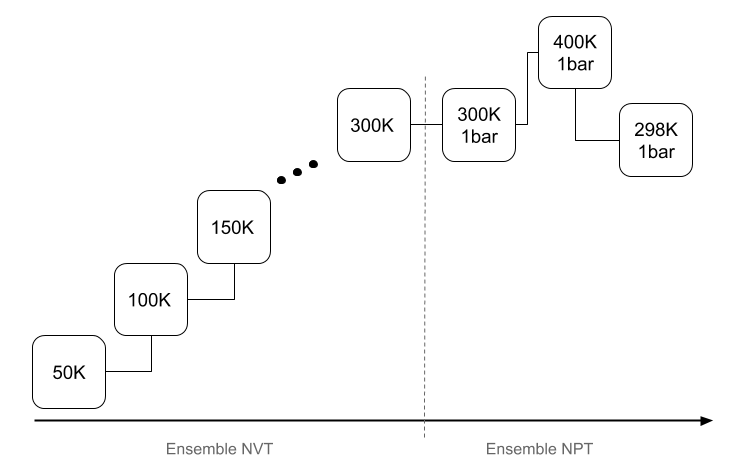
\includegraphics[scale=0.6]{equilib.png}
\caption{Rampa de temperatura considerada para a equilibração do sistema. Cada um dos ciclos foi simulado por 200 ps.}
\label{equilib}
\end{figure}

A equilibração dos sistemas foi realizada em um ensemble NVT onde a temperatura foi elevada gradadivamente segundo um perfil de escada para evitar uma movimentação que pudesse levar à superposições de volumes atômicos e consequente divergência do sistema.
Velocidades iniciais foram geradas segundo uma distribuição de Maxwell-Boltzmann correspondente à temperatura de 50K.
Então, seis equilibrações sucessivas de 200 ps foram realizadas aumentando gradualmente a temperatura de 50 a 300 K em intervalos de 50K (Figura \ref{equilib}).
Após isso, a equilibração foi continuada no ensemble NPT controlando a pressão em 1 bar.
A fim de remover influências da estrutura inicial, o sistema foi levado até 400K e simulado por 200 ps antes de ser resfriado a 298.15 K por mais 200 ps (Figura \ref{equilib}).
Essa equilibração lenta é particularmente importante para os dendrímeros de gerações mais altas devido a sua estrutura altamente complexa.

Após a equilibração, 50 ns de dinâmica molecular foram feitos com a configuração descrita acima. 
Para garantir que as propriedades fossem calculadas em uma janela de tempo onde elas já haviam convergido, os últimos 10 ns foram utilizados para o cálculo das propriedades para a validação e estudo dos sistemas.
O raio de giro e as funções de distribuição radial foram calculadas com rotinas nativas do gromacs-5.1.4 enquanto os fatores de forma e as asfericidades, com um script escrito pelos autores por motivos que serão melhor discutidos nas Seções \ref{PAMAMForma} e \ref{PPIForma}.

\pagebreak
